\documentclass[11pt,journal,draftclsnofoot,onecolumn]{IEEEtran}
% NOTE: this is the one-column "draft" mode of IEEEtran (double spaced), which is how
% IEEE journals ask for review drafts. To see the final two-column layout, replace the
% line above by:  \documentclass[conference]{IEEEtran}

\usepackage[T1]{fontenc}
\usepackage[utf8]{inputenc}
\usepackage{cite}
\usepackage{amsmath,amssymb,amsfonts}
\usepackage{graphicx}
\usepackage{booktabs}
\usepackage{array}
\usepackage{textcomp}
\usepackage{url}
\graphicspath{{figures/}}

% Optional figures: only included if you copy the PNG from your own notebook into figures/
\newcommand{\optfig}[4]{\IfFileExists{figures/#1}{\begin{figure}[!t]\centering
  \includegraphics[width=#2\linewidth]{figures/#1}\caption{#3}\label{#4}\end{figure}}{}}
\newcommand{\optsent}[3]{\IfFileExists{figures/#1}{#2}{#3}}

\begin{document}

\title{Drivers of Guest Satisfaction in European Hotels: Combining TF-IDF Sentiment Classification and LDA Topic Modelling on 515,000 Online Reviews}

\author{\IEEEauthorblockN{[Your Name]}
\IEEEauthorblockA{[Master's Programme, University]\\
\relax[City], Germany\\
Email: [your.email@university.edu]}}

\maketitle

\begin{abstract}
Online reviews are a large and continuously growing source of customer feedback, yet hotels rarely turn them into systematic evidence about what makes guests satisfied or dissatisfied. This paper presents a scalable, reproducible text-analytics pipeline that identifies the main drivers of guest satisfaction in European hotels. Using 515,738 Booking.com reviews, we split each review into its positive and negative text fields, which yields 862,958 labelled text segments after cleaning. We compare Naive Bayes, Logistic Regression and Linear SVM classifiers on TF-IDF uni- and bigram features, and fit separate Latent Dirichlet Allocation (LDA) models to positive ($k=13$) and negative ($k=9$) texts, with $k$ selected by $c_v$ topic coherence. Topics from both models are mapped to shared themes and their prevalence is compared across sentiment groups. Logistic Regression achieved the best held-out macro-F1 (0.929), ahead of Linear SVM (0.925) and Naive Bayes (0.918). Room quality (30.2\% of complaints versus 10.6\% of praise) and breakfast and food (18.8\% versus 5.4\%) are strongly over-represented in negative texts, as are noise and check-in issues, whereas location (29.8\% of praise versus 7.4\% of complaints) is the dominant source of positive sentiment. Staff and service is prominent in both groups. The results separate hygiene factors from satisfaction drivers and indicate where hotels can reduce complaints most effectively. We discuss the limits of structure-derived labels and outline extensions to Spark-based processing and transformer models.
\end{abstract}

\begin{IEEEkeywords}
sentiment analysis, topic modelling, latent Dirichlet allocation, TF-IDF, online reviews, hospitality analytics, customer satisfaction
\end{IEEEkeywords}

\section{Introduction}
\IEEEPARstart{O}{nline} travel platforms have changed how guests choose hotels and how hotels learn from their guests. Reviews are written in free text, arrive continuously and, unlike surveys, are unsolicited. Prior work shows that travellers rely heavily on such content when planning trips \cite{xiang2010} and that review valence is associated with hotel performance \cite{ye2009}. For a hotel manager, the practical problem is not a lack of feedback but its volume: a single large property receives thousands of comments per year and a hotel chain receives millions. Reading them manually is infeasible, and a star rating alone says little about \emph{why} a guest was satisfied or dissatisfied.

\subsection{Business Context and Motivation in Big Data Analytics}
Hotel review analysis is a typical big-data analytics problem. The data are unstructured text (volume), arrive continuously from many platforms (velocity), mix vocabularies, languages and writing styles (variety) and carry noisy, self-reported judgements (veracity). Turning this raw material into decisions requires a pipeline that cleans and normalises text, represents it numerically, extracts both an evaluative signal (sentiment) and a descriptive signal (what the guest talks about), and combines them into a form that a non-technical manager can act on. The corpus used in this study, about half a million reviews, is moderate in size for a single machine but already exhibits the scaling issues of larger deployments: very high-dimensional sparse feature matrices, long-running probabilistic inference, and the need to persist intermediate results so that expensive steps are not repeated.

\subsection{Research Gap}
Existing studies typically (i) apply sentiment classification or topic modelling in isolation, (ii) fit a single topic model on all text so that the vocabulary of praise and the vocabulary of complaints are blended into the same topics, or (iii) analyse small samples from a single city or platform. Few studies describe the computational design choices needed to run the complete analysis on a corpus of several hundred thousand reviews, or discuss how the resulting topics can be compared across sentiment groups when two separate topic models are used.

\subsection{Research Questions and Contributions}
This paper addresses three research questions:
\begin{itemize}
\item \textbf{RQ1:} How accurately can the polarity of a hotel review text be predicted from TF-IDF features, and how do Naive Bayes, Logistic Regression and Linear SVM compare in accuracy and training cost?
\item \textbf{RQ2:} Which themes do guests discuss when they praise and when they complain, and how many topics are needed to describe each group?
\item \textbf{RQ3:} Which themes are disproportionately associated with negative or with positive texts, i.e. which behave as hygiene factors and which as satisfaction drivers?
\end{itemize}
The contributions are: (1) a reproducible end-to-end pipeline from raw review data to managerial insight; (2) a systematic comparison of three classical classifiers on large-scale review text, including training cost; (3) sentiment-specific LDA models with coherence-based selection of the number of topics, and a theme-harmonisation step that makes the two topic models comparable; (4) empirical findings on which aspects of the hotel experience are most strongly associated with complaints and with praise; and (5) a discussion of failure modes, scalability and industrial deployment. All code is released in a public repository.

\subsection{Organisation}
Section~II reviews related work. Section~III describes the data and preprocessing. Section~IV presents the methodology and system framework. Section~V details the experimental setup. Section~VI reports results, Section~VII discusses implications, scalability and limitations, and Section~VIII concludes.

\section{Related Work}
\subsection{Online Reviews in Hospitality Research}
Xiang and Gretzel documented the growing role of social media content in travel information search \cite{xiang2010}, and Ye et al.\ linked online review valence to hotel room sales \cite{ye2009}. These studies establish the commercial importance of reviews but mostly rely on star ratings or aggregate scores. Guo et al.\ went further and applied LDA to hotel reviews to identify the dimensions of tourist satisfaction \cite{guo2017}, demonstrating that topic models can recover interpretable service dimensions from free text. Our work builds on this line but fits separate models to positive and negative text and quantifies how theme prevalence differs between them.

\subsection{Sentiment Classification}
Pang et al.\ showed that supervised machine learning outperforms rule-based baselines for sentiment classification of movie reviews \cite{pang2002}. For text, linear models on sparse bag-of-words features remain strong baselines: support vector machines handle the high dimensionality and sparsity of text well \cite{joachims1998}, multinomial Naive Bayes is fast and competitive on short texts \cite{mccallum1998}, and Wang and Manning showed that Naive Bayes and SVM variants using bigram features are hard to beat on many sentiment tasks \cite{wang2012}. Term frequency--inverse document frequency (TF-IDF) weighting \cite{salton1988} is the standard feature representation for such models. Comprehensive overviews are given by Liu \cite{liu2012}. Pre-trained transformer models such as BERT \cite{devlin2019} now achieve higher accuracy on many benchmarks, but they require considerably more computation and are therefore left for future work; the linear models studied here remain attractive when interpretability and training cost matter.

\subsection{Topic Modelling}
Latent Dirichlet Allocation (LDA) \cite{blei2003} models each document as a mixture of latent topics and each topic as a distribution over words; Blei gives an accessible review \cite{blei2012}. Online variational Bayes \cite{hoffman2010} makes inference feasible for large corpora and is the algorithm implemented in the Gensim library \cite{rehurek2010}. Because LDA does not tell the analyst how many topics to use, topic quality is commonly assessed with coherence measures that correlate with human judgement. UMass coherence \cite{mimno2011} and the $c_v$ measure studied by R\"oder et al.\ \cite{roder2015} are widely used.

\subsection{Hygiene Factors and Satisfaction Drivers}
Herzberg's two-factor theory distinguishes hygiene factors, whose absence or poor quality causes dissatisfaction but whose presence does not create satisfaction, from motivators that create satisfaction \cite{herzberg1959}. Although originally developed for workplace motivation, the distinction is useful for service settings: it predicts that some aspects of a hotel stay are mentioned mainly when they fail, while others are mentioned mainly when they delight. Comparing the prevalence of themes in negative and positive text offers a data-driven way to examine this distinction.

\subsection{Summary of the Gap}
The literature provides each ingredient separately, but a compact, reproducible study that (a) compares classical classifiers on a half-million-review corpus, (b) fits sentiment-specific topic models with coherence-based model selection, and (c) harmonises the resulting topics into shared themes for a direct, quantitative comparison is still uncommon. This paper provides such a study.

\section{Data and Preprocessing}
\subsection{Dataset}
We use the public ``515K Hotel Reviews Data in Europe'' dataset \cite{liu2018dataset}, which contains 515,738 customer reviews scraped from Booking.com for about 1,500 hotels in six countries (Austria, France, Italy, the Netherlands, Spain and the United Kingdom), written between 2015 and 2017. Each record contains the hotel name and address, review date, reviewer nationality, an overall reviewer score between 2.5 and 10, and two free-text fields: a \emph{positive} review field and a \emph{negative} review field. The data are public and were already available before this study; we do not attempt to identify individual reviewers.

\subsection{Label Construction}
Manual annotation of several hundred thousand texts is infeasible. We therefore use the \emph{structure} of the review form as a weak label: text written in the positive field is labelled \emph{positive}, and text written in the negative field is labelled \emph{negative}. A single review can therefore contribute up to two labelled segments, and the data are reshaped from a wide format (one row per review) into a long format (one row per text segment). The platform inserts the placeholders ``No Positive'' and ``No Negative'' when a field is left empty; these placeholders are not text and are removed before any language processing. The negative field was left empty in 127,890 reviews (24.8\%). As a sanity check, the distribution of the overall reviewer score was compared between the two label groups (notebook 01 in the repository).

\subsection{Cleaning and Normalisation Pipeline}
Preprocessing follows a fixed sequence, implemented as the first notebook of the repository:
\begin{enumerate}
\item parse review dates and extract the hotel country from the address string, with an explicit rule for United Kingdom addresses, which do not end in the country name in the same way as other addresses;
\item remove placeholder strings and build the long-format table of labelled segments;
\item convert text to lower case and replace all non-alphabetic characters by spaces;
\item remove English stop words (NLTK list) and tokens of two characters or fewer;
\item lemmatise tokens with the WordNet lemmatiser \cite{bird2009};
\item drop segments that are empty after cleaning;
\item for topic modelling only, remove 20 additional high-frequency domain words (e.g. ``hotel'', ``room'', ``stay'', ``night'') that appear in nearly every review and would otherwise dominate every topic.
\end{enumerate}
The raw text is retained in a separate column for error inspection. Intermediate results are stored in columnar Parquet files so that each downstream notebook starts from a verified checkpoint.

\begin{table}[!t]
\caption{Dataset after preprocessing}
\label{tab:data}
\centering
\begin{tabular}{lrr}
\toprule
Stage & Positive & Negative \\
\midrule
Reviews with usable text field before cleaning & -- & 387,848 \\
Text segments after cleaning & 478,843 & 384,115 \\
Share of all labelled segments & 55.5\% & 44.5\% \\
\midrule
Total labelled segments & \multicolumn{2}{c}{862,958} \\
\bottomrule
\end{tabular}
\end{table}

Table~\ref{tab:data} summarises the result. The classes are moderately imbalanced (55.5\% positive), so macro-averaged F1 is reported alongside accuracy and class weighting is used for the linear models.

\section{Methodology and System Framework}
\subsection{Framework Overview}
Fig.~\ref{fig:pipeline} shows the framework. After ETL and cleaning, the labelled text follows two parallel branches that share the same normalised text. The \emph{sentiment branch} converts text into TF-IDF vectors and trains and evaluates three classifiers. The \emph{topic branch} builds a dictionary and bag-of-words corpus and fits one LDA model for each sentiment group. The branches are joined in a combined analysis in which topics are mapped to shared themes and their prevalence is compared across sentiments. Because every stage writes its output to disk, the stages are decoupled and can be re-run independently, which matters when individual steps (such as LDA tuning) take tens of minutes.

\begin{figure}[!t]
\centering
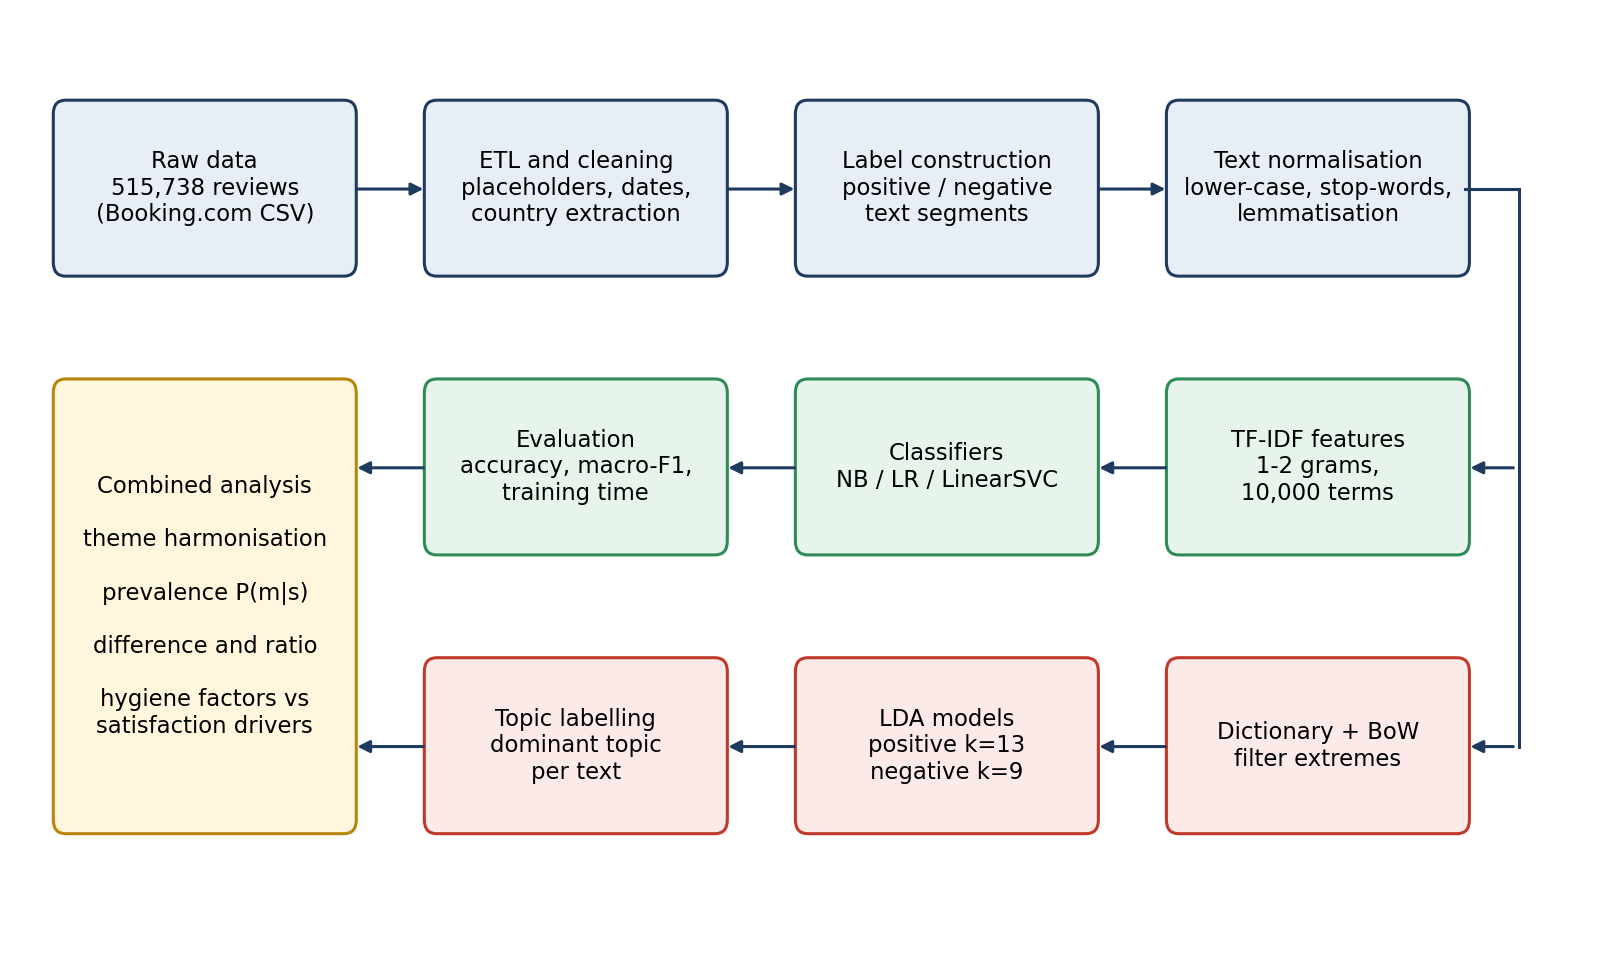
\includegraphics[width=0.92\linewidth]{fig_pipeline.png}
\caption{System framework: from raw reviews to managerial insight. The sentiment branch (green) and topic branch (red) share the normalised text and are joined in the combined analysis.}
\label{fig:pipeline}
\end{figure}

\subsection{Feature Engineering: TF-IDF}
Each cleaned segment $d$ is represented as a sparse vector of TF-IDF weights. With $N$ segments and document frequency $\mathrm{df}(t)$ of term $t$,
\begin{equation}
\mathrm{tfidf}(t,d)=\mathrm{tf}(t,d)\left(\ln\frac{1+N}{1+\mathrm{df}(t)}+1\right),
\end{equation}
and each vector is $L_2$-normalised, $\mathbf{x}_d=\mathbf{v}_d/\lVert\mathbf{v}_d\rVert_2$. Unigrams and bigrams are used so that short phrases such as ``very clean'' or ``too small'' are captured. The vocabulary is limited to the 10,000 highest-frequency terms, terms in fewer than 5 segments or more than 90\% of segments are discarded, and the vectoriser is fitted on the training split only to avoid information leakage into the test set.

\subsection{Classifiers}
\subsubsection{Multinomial Naive Bayes}
Naive Bayes assigns a segment to the class with the highest posterior under a conditional independence assumption \cite{mccallum1998}:
\begin{equation}
\hat{y}=\arg\max_{c\in\{+,-\}}\Big[\ln P(c)+\sum_{t\in V}x_{t}\ln P(t\mid c)\Big],\quad
P(t\mid c)=\frac{N_{tc}+\alpha}{\sum_{t'}N_{t'c}+\alpha|V|},
\end{equation}
where $N_{tc}$ is the weight mass of term $t$ in class $c$ and $\alpha=1$ is Laplace smoothing.

\subsubsection{Logistic Regression}
Logistic Regression models $P(y=+\mid\mathbf{x})=\sigma(\mathbf{w}^{\top}\mathbf{x}+b)$ and minimises the $L_2$-regularised logistic loss
\begin{equation}
\min_{\mathbf{w},b}\ \tfrac12\lVert\mathbf{w}\rVert_2^2+C\sum_{i}s_i\ln\!\big(1+e^{-y_i(\mathbf{w}^{\top}\mathbf{x}_i+b)}\big),
\end{equation}
with labels $y_i\in\{-1,+1\}$ and class weights $s_i=N/(2N_{c(i)})$ (``balanced''), where $N_{c(i)}$ is the number of training segments in the class of segment $i$.

\subsubsection{Linear Support Vector Machine}
The linear SVM \cite{joachims1998} replaces the logistic loss by the squared hinge loss, which in the implementation used here is solved by the LIBLINEAR library \cite{fan2008}:
\begin{equation}
\min_{\mathbf{w},b}\ \tfrac12\lVert\mathbf{w}\rVert_2^2+C\sum_{i}s_i\max\!\big(0,\,1-y_i(\mathbf{w}^{\top}\mathbf{x}_i+b)\big)^2 .
\end{equation}

\subsection{Topic Modelling with LDA}
LDA assumes that each segment $d$ has a topic mixture $\boldsymbol{\theta}_d\sim\mathrm{Dir}(\alpha)$, each topic $k$ has a word distribution $\boldsymbol{\varphi}_k\sim\mathrm{Dir}(\eta)$, and each word is generated by drawing a topic $z_{d,n}\sim\mathrm{Cat}(\boldsymbol{\theta}_d)$ and then a word $w_{d,n}\sim\mathrm{Cat}(\boldsymbol{\varphi}_{z_{d,n}})$ \cite{blei2003}. The posterior is approximated by online variational Bayes \cite{hoffman2010} using Gensim \cite{rehurek2010}.

Two design decisions are central. First, \emph{separate models are fitted to positive and negative segments}, because guests praise and complain about different things, and a single model would blend these vocabularies. Second, the number of topics $k$ is selected for each model with the $c_v$ coherence measure \cite{roder2015}, which uses normalised pointwise mutual information (NPMI) between top words,
\begin{equation}
\mathrm{NPMI}(w_i,w_j)=\frac{\ln\frac{P(w_i,w_j)}{P(w_i)P(w_j)}}{-\ln P(w_i,w_j)},
\end{equation}
estimated in a sliding window over the corpus, and compares the resulting context vectors by cosine similarity. For each $k\in\{5,7,9,11,13,15\}$ a model is trained and its coherence recorded, and $k$ is set to the value with the highest score. Each topic is then labelled manually from its ten highest-weight words, and each segment is assigned its dominant topic $z_d^{*}=\arg\max_k\theta_{d,k}$.

\subsection{Combined Analysis: From Topics to Themes}
Because the two LDA models are independent, their topics are not directly comparable (a ``breakfast'' topic exists in both, but with different labels and word weights). We therefore map the manually labelled topics of both models onto a common set of \emph{themes} (Table~\ref{tab:themes}). Let $N_{s,m}$ be the number of segments of sentiment $s$ assigned to theme $m$. The prevalence of theme $m$ within sentiment $s$, the difference between sentiments, and the ratio are
\begin{align}
P(m\mid s)&=100\cdot\frac{N_{s,m}}{\sum_{m'}N_{s,m'}},\\
\Delta_m&=P(m\mid -)-P(m\mid +),\qquad R_m=\frac{P(m\mid -)}{P(m\mid +)} .
\end{align}
A large positive $\Delta_m$ indicates a theme that is over-represented in complaints (a hygiene-factor candidate), and a large negative $\Delta_m$ a theme over-represented in praise (a satisfaction-driver candidate). The measure is a share \emph{within} each sentiment group: $P(m\mid -)=30\%$ means that 30\% of complaint texts are mainly about theme $m$, not that 30\% of guests complained about it.

\begin{table}[!t]
\caption{Mapping of topics to shared themes}
\label{tab:themes}
\centering
\small
\begin{tabular}{p{2.6cm}p{5.4cm}p{5.4cm}}
\toprule
Theme & Positive-model topics & Negative-model topics \\
\midrule
Location & General location; transit access; nearby amenities & Location (distance) \\
Staff \& Service & Staff friendliness; service \& facilities & Staff \& booking issues \\
Room & Room comfort & Bed size/comfort \& parking; bathroom condition \\
Breakfast \& Food & Breakfast quality & Breakfast, food \& price \\
Ambiance \& Facilities & View \& ambiance; extras/perks & Heating/AC \& maintenance \\
Value \& Price & Value for money & -- (absorbed in Breakfast, food \& price) \\
Noise & -- & Noise \\
Check-in \& Payments & -- & Check-in, WiFi \& payment \\
General Praise & Overall experience; recommendation & -- \\
Other & Minor/mixed remarks & -- \\
\emph{Excluded} & -- & ``No complaint'' filler topic \\
\bottomrule
\end{tabular}
\end{table}

One negative-model topic is dominated by words such as ``nothing'', ``everything'', ``great'' and ``perfect''. It captures guests who wrote ``Nothing to complain about'' in the negative field and is not a complaint; it is excluded from the combined analysis (Section~VI-D).

\subsection{Computational Considerations}
Constructing TF-IDF vectors and fitting Naive Bayes both scale linearly with the number of non-zero entries of the sparse matrix; Logistic Regression and the linear SVM require several passes over the same matrix. LDA is considerably more expensive, with a cost per pass proportional to the number of tokens times $k$, and was the dominant computational cost of this study. Three measures keep the workflow tractable on a single CPU: development of classifiers on a stratified random sample before retraining the selected model on the full corpus; tuning of LDA on subsampled corpora and applying the trained models to all segments (inference is much cheaper than training); and persisting vectorisers, dictionaries, models and topic assignments to disk.

\section{Experimental Setup}
\subsection{Environment and Data Split}
All experiments ran on a standard Windows laptop (CPU only, no GPU) using Python with pandas, scikit-learn \cite{pedregosa2011}, Gensim \cite{rehurek2010}, NLTK \cite{bird2009} and matplotlib. Random seeds are fixed (42). For model comparison, a random sample of 150,000 segments was drawn from the 862,958 labelled segments and split 80/20 into 120,000 training and 30,000 test segments, stratified by label. The TF-IDF vectoriser was fitted on the training segments only. The selected classifier was subsequently retrained on the full corpus and used to label every segment.

\subsection{Hyperparameters}
Table~\ref{tab:hyper} lists the settings. No extensive hyperparameter search was performed for the classifiers; library defaults were used for regularisation strength, because the aim of RQ1 is a comparison of well-understood baselines rather than maximum accuracy.

\begin{table}[!t]
\caption{Model settings}
\label{tab:hyper}
\centering
\small
\begin{tabular}{p{3.1cm}p{9cm}}
\toprule
Component & Setting \\
\midrule
TF-IDF & 1--2-grams, 10,000 features, min\_df $=5$, max\_df $=0.9$, $L_2$ norm \\
Naive Bayes & multinomial, $\alpha=1.0$ \\
Logistic Regression & $L_2$ penalty, $C=1$, balanced class weights, max 1,000 iterations \\
Linear SVM & squared hinge loss, $L_2$ penalty, $C=1$, balanced class weights \\
LDA dictionary & terms in at least 5 and at most 50\% of segments \\
LDA training & online variational Bayes, symmetric priors, 10 passes for the final models, fixed seed \\
LDA selection & $k\in\{5,7,9,11,13,15\}$, $c_v$ coherence \\
\bottomrule
\end{tabular}
\end{table}

\subsection{Evaluation Metrics}
Classification is evaluated with accuracy, per-class precision and recall, and macro-averaged F1,
\begin{equation}
\mathrm{F1}_c=\frac{2P_cR_c}{P_c+R_c},\qquad \text{macro-F1}=\frac{1}{2}\sum_{c\in\{+,-\}}\mathrm{F1}_c,
\end{equation}
together with the wall-clock model fitting time. Because the test set contains $n=30{,}000$ segments, the 95\% binomial confidence half-width of an accuracy near 0.93 is $1.96\sqrt{p(1-p)/n}\approx0.003$ (0.3 percentage points), which is used to judge whether differences between models are meaningful. Topic models are evaluated by $c_v$ coherence for model selection and by manual inspection of the top words of each topic. The combined analysis is evaluated through the interpretability and stability of the theme-level contrasts $\Delta_m$ and $R_m$.

\subsection{Evaluation Data}
All experiments use the real-world Booking.com corpus described in Section~III. No synthetic data were used. Failure modes considered in advance include label noise from structure-derived labels, loss of negation during stop-word removal, redundant or catch-all topics, one-sided themes caused by using two topic models, and limited temporal and geographic coverage. They are examined in Section~VI-D.

\section{Results}
\subsection{Sentiment Classification (RQ1)}
Table~\ref{tab:clf} and Fig.~\ref{fig:clf} show the results on the held-out test split. All three models achieve more than 91\% accuracy, so TF-IDF with linear or probabilistic classifiers separates the two text types well. Logistic Regression is the best model on both metrics (accuracy 0.9286, macro-F1 0.9286). Linear SVM follows closely (0.9261 and 0.9254), and Naive Bayes is about one percentage point behind (0.9194 and 0.9183).

\begin{table}[!t]
\caption{Sentiment classification results on the held-out test split ($n=30{,}000$)}
\label{tab:clf}
\centering
\begin{tabular}{lccc}
\toprule
Model & Accuracy & Macro-F1 & Fit time (s) \\
\midrule
Multinomial Naive Bayes & 0.9194 & 0.9183 & \textbf{0.26} \\
Logistic Regression & \textbf{0.9286} & \textbf{0.9286} & 0.80 \\
Linear SVM & 0.9261 & 0.9254 & 1.64 \\
\bottomrule
\end{tabular}
\end{table}

\begin{figure}[!t]
\centering
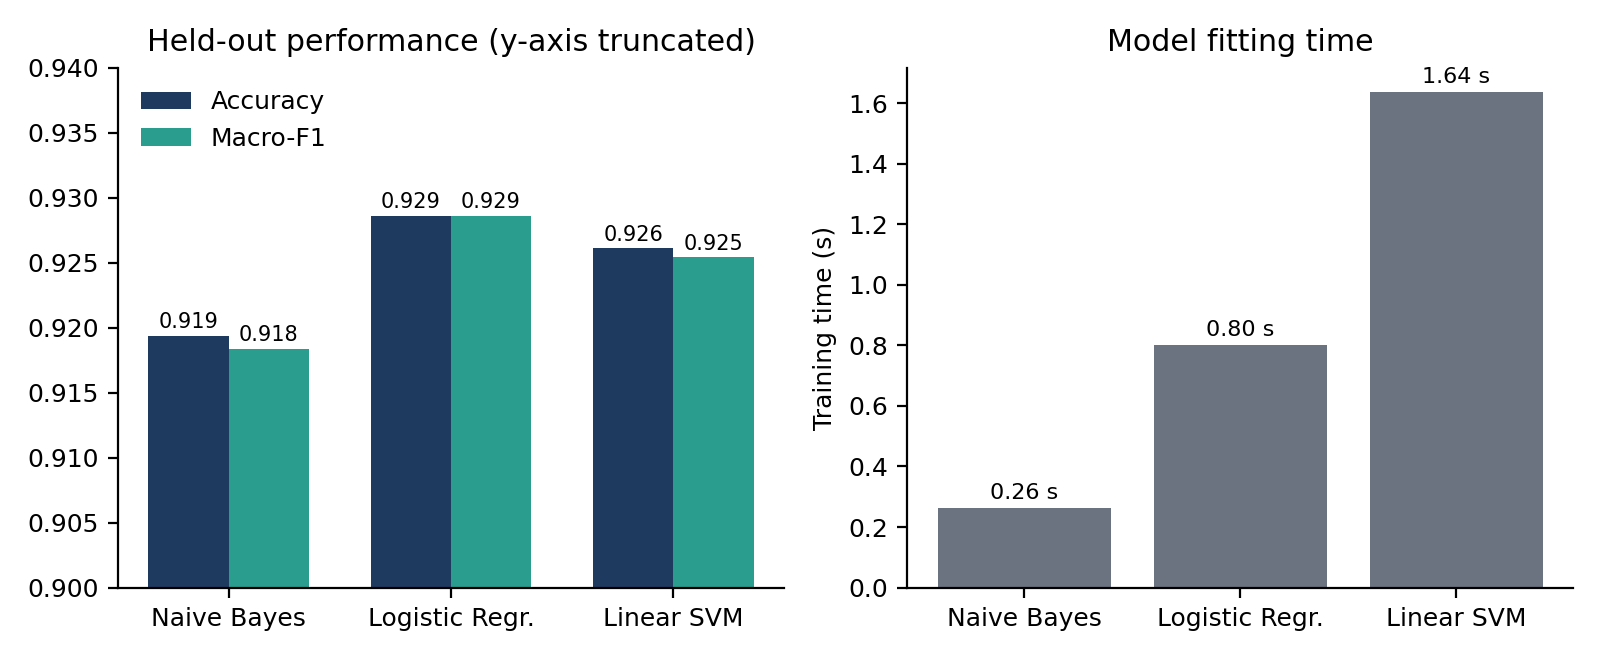
\includegraphics[width=0.95\linewidth]{fig_model_comparison.png}
\caption{Left: accuracy and macro-F1 of the three classifiers (y-axis truncated to 0.90--0.94 for readability). Right: model fitting time.}
\label{fig:clf}
\end{figure}

The gap between Logistic Regression and Naive Bayes (about 0.9 percentage points in accuracy and 1.0 in macro-F1) is larger than the sampling uncertainty of roughly $\pm0.3$ points and is therefore meaningful. The gap between Logistic Regression and the linear SVM (0.25 points in accuracy) is of the same order as that uncertainty, so we do not claim that Logistic Regression is significantly better than the SVM; we observe only that the SVM brings no advantage here. The common expectation that an SVM is the strongest linear classifier for sparse text is thus not borne out on this data, while Logistic Regression is also about twice as fast to fit. The cost ordering is clear: Naive Bayes is the fastest, Logistic Regression roughly three times and the SVM roughly six times slower. Naive Bayes is therefore a sensible choice when training time dominates, and Logistic Regression is the best compromise.
\optsent{sentiment_confusion_matrices.png}{Fig.~\ref{fig:cm} shows the confusion matrices of the three models.}{}

\optfig{sentiment_confusion_matrices.png}{0.98}{Confusion matrices of the three classifiers on the test split.}{fig:cm}

An important caveat for interpretation: the labels are derived from the review form, so the classifier has learned to predict which field a text was written in. Its accuracy shows that the two kinds of text have distinct vocabularies, but it should not be read as accuracy on independently annotated sentiment (see Section~VII-E).

\subsection{Topic Models (RQ2)}
Fig.~\ref{fig:coh} shows the coherence sweep. For positive texts, coherence rises from 0.627 at $k=7$ to a maximum of 0.6455 at $k=13$ and then drops to 0.633 at $k=15$. For negative texts, it peaks sharply at $k=9$ (0.7213) and declines steadily for larger $k$ (0.7134, 0.7034, 0.6957). The different optima are plausible: positive texts cover many distinct themes (location in several forms, staff, breakfast, views, value), while complaints concentrate on fewer recurring issues, so additional topics merely split the same complaint. Raw coherence values should not be compared across the two corpora, only across $k$ within one corpus.

\begin{figure}[!t]
\centering
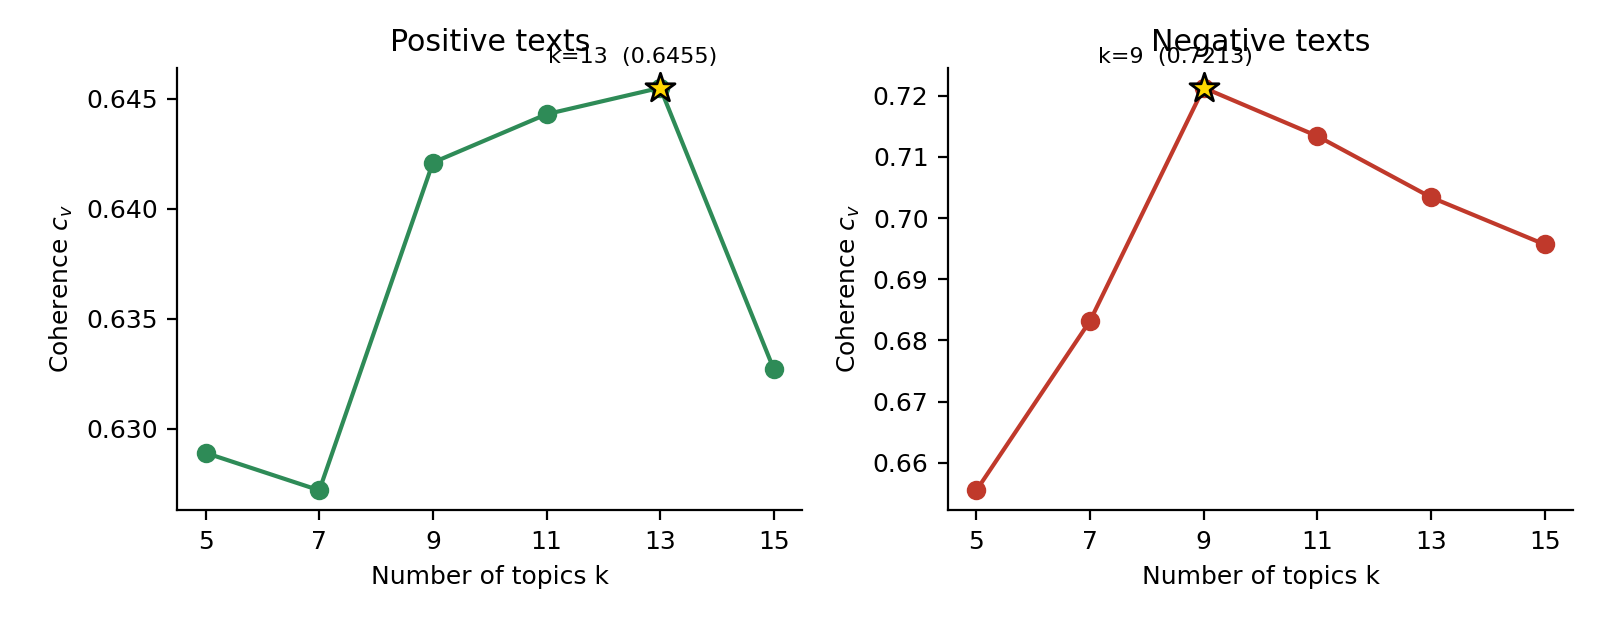
\includegraphics[width=0.98\linewidth]{fig_coherence.png}
\caption{$c_v$ coherence as a function of the number of topics $k$ for positive (left) and negative (right) texts. Stars mark the selected $k$.}
\label{fig:coh}
\end{figure}

The practical value of the sweep was visible in an early trial. A model with $k=10$, chosen arbitrarily and not tested by the sweep, produced two topics that were both dominated by ``station'', ``metro'' and ``close'', together with a weakly defined catch-all topic. With the coherence-selected $k=13$, location is split into three distinct and interpretable aspects (general location praise, transit access, and nearby restaurants and walking distance), and breakfast and value for money are separated. Tables~\ref{tab:postopics} and~\ref{tab:negtopics} list the final topics.

\begin{table}[!t]
\caption{Positive-text topics ($k=13$): label, highest-weight words and number of segments}
\label{tab:postopics}
\centering
\footnotesize
\begin{tabular}{p{4.0cm}p{7.4cm}r}
\toprule
Topic label & Top words & Segments \\
\midrule
Staff friendliness & staff, friendly, helpful, location, clean, breakfast & 96,394 \\
Location (general) & great, location, excellent, design, central, convenient & 53,512 \\
Location -- transit access & station, close, metro, city, walk, easy, near, train & 52,059 \\
Room comfort & bed, comfortable, clean, bathroom, comfy, spacious, modern & 50,903 \\
Location -- nearby amenities & restaurant, walking, distance, area, pool, located, street & 37,174 \\
Value for money & good, location, breakfast, value, money, price, wifi & 35,404 \\
View \& ambiance & view, bar, staff, lovely, beautiful, new, decor & 28,331 \\
Extras/perks & free, check, drink, car, upgrade, early, reception, birthday & 26,885 \\
Breakfast quality & breakfast, nice, choice, coffee, buffet, delicious, fresh & 25,734 \\
Service \& facilities & service, staff, excellent, food, facility, restaurant, desk & 23,833 \\
Recommendation/repeat visit & time, best, definitely, recommend, back, every & 17,272 \\
Overall experience & everything, perfect, amazing, loved, spa, style & 16,707 \\
Minor/mixed remarks (weak) & well, like, nothing, small, old, liked, little, building & 14,635 \\
\bottomrule
\end{tabular}
\end{table}

\begin{table}[!t]
\caption{Negative-text topics ($k=9$): label, highest-weight words and number of segments}
\label{tab:negtopics}
\centering
\footnotesize
\begin{tabular}{p{4.0cm}p{7.4cm}r}
\toprule
Topic label & Top words & Segments \\
\midrule
Breakfast, food \& price & breakfast, bar, price, coffee, expensive, food, restaurant & 64,388 \\
Bathroom condition & bathroom, shower, old, small, toilet, dirty, water & 52,024 \\
Bed size/comfort \& parking & bed, small, parking, double, hard, pillow, car & 51,407 \\
Staff \& booking issues & staff, reception, booking, asked, told, booked & 50,131 \\
``No complaint'' filler (excluded) & nothing, everything, bad, great, like, perfect, complaint & 41,800 \\
Noise & noise, noisy, floor, door, window, outside, street, lift & 40,585 \\
Check-in, WiFi \& payment & check, wifi, time, pay, free, hour, card, long & 35,971 \\
Location (distance) & location, pool, far, city, walk, station, area & 25,269 \\
Heating/AC \& maintenance & air, hot, cold, conditioning, working, window, water & 22,537 \\
\bottomrule
\end{tabular}
\end{table}

The negative topics are specific and actionable: bathroom condition, bed size and comfort, breakfast and its price, noise, check-in and WiFi, heating and air conditioning, and staff or booking problems. Three negative segments received no topic assignment and were dropped from the topic analysis.

\subsection{Combined Analysis (RQ3)}
After removing the 41,800 filler segments (10.9\% of negative segments), 342,312 negative and 478,843 positive segments remain. Table~\ref{tab:combined} and Figs.~\ref{fig:themes} and~\ref{fig:diff} give the theme prevalence per sentiment group.

\begin{table}[!t]
\caption{Theme prevalence within each sentiment group (\%), difference $\Delta_m$ and ratio $R_m$}
\label{tab:combined}
\centering
\begin{tabular}{lrrrr}
\toprule
Theme & Positive & Negative & $\Delta_m$ & $R_m$ \\
\midrule
Room & 10.63 & 30.22 & +19.59 & 2.84 \\
Breakfast \& Food & 5.37 & 18.81 & +13.44 & 3.50 \\
Noise & 0.00 & 11.86 & +11.86 & -- \\
Check-in \& Payments & 0.00 & 10.51 & +10.51 & -- \\
Other & 3.06 & 0.00 & $-3.06$ & 0.00 \\
Ambiance \& Facilities & 11.53 & 6.58 & $-4.95$ & 0.57 \\
General Praise & 7.10 & 0.00 & $-7.10$ & 0.00 \\
Value \& Price & 7.39 & 0.00 & $-7.39$ & 0.00 \\
Staff \& Service & 25.11 & 14.64 & $-10.46$ & 0.58 \\
Location & 29.81 & 7.38 & $-22.43$ & 0.25 \\
\bottomrule
\end{tabular}
\end{table}

\begin{figure}[!t]
\centering
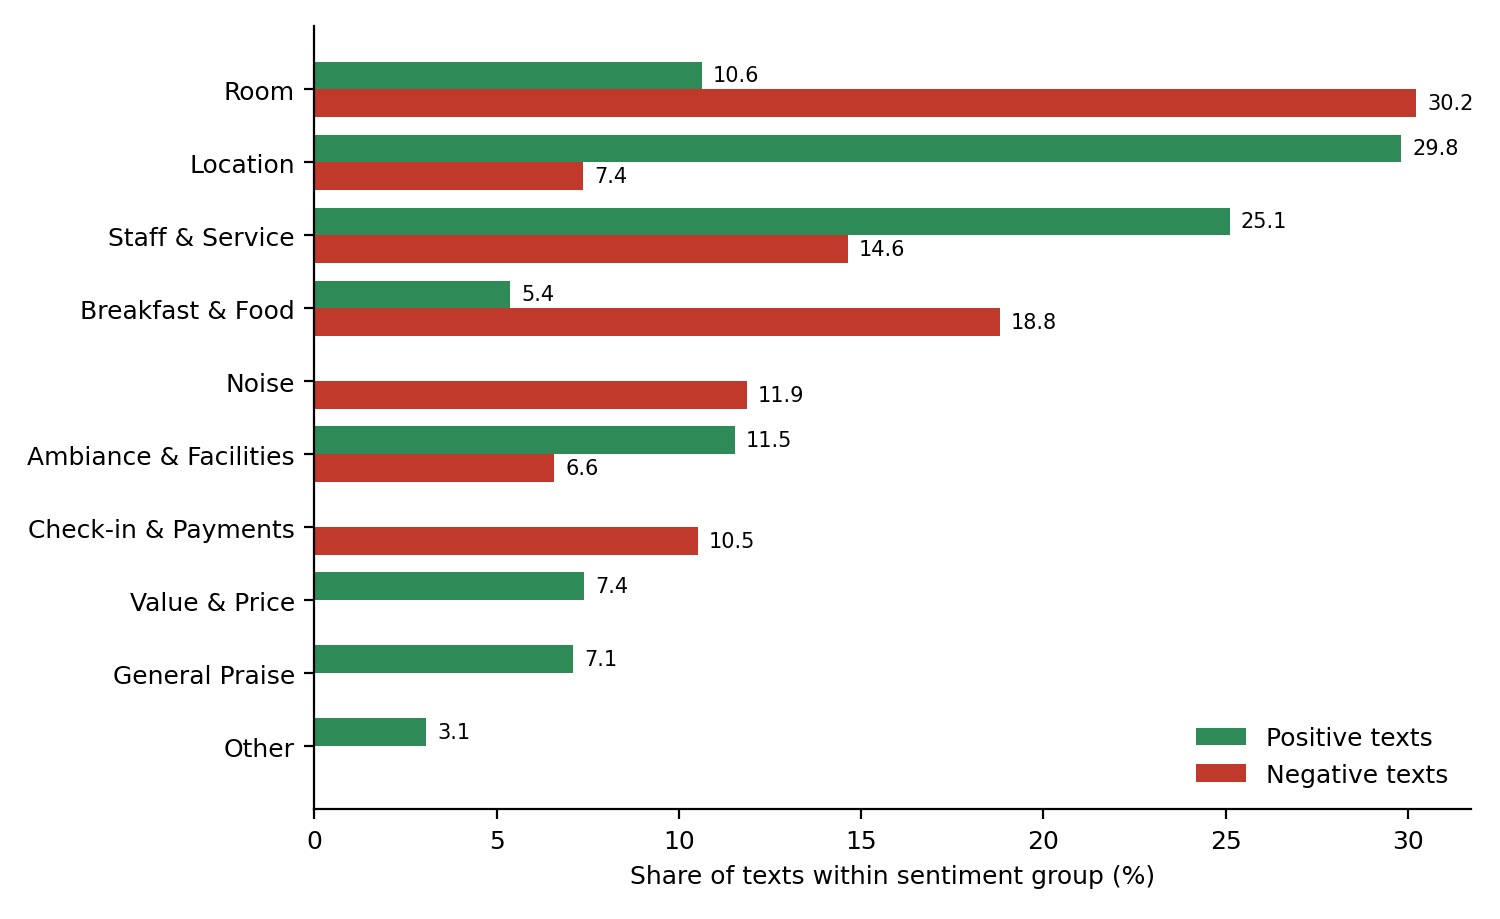
\includegraphics[width=0.92\linewidth]{fig_theme_comparison.png}
\caption{Share of texts within each sentiment group assigned to each theme.}
\label{fig:themes}
\end{figure}

\begin{figure}[!t]
\centering
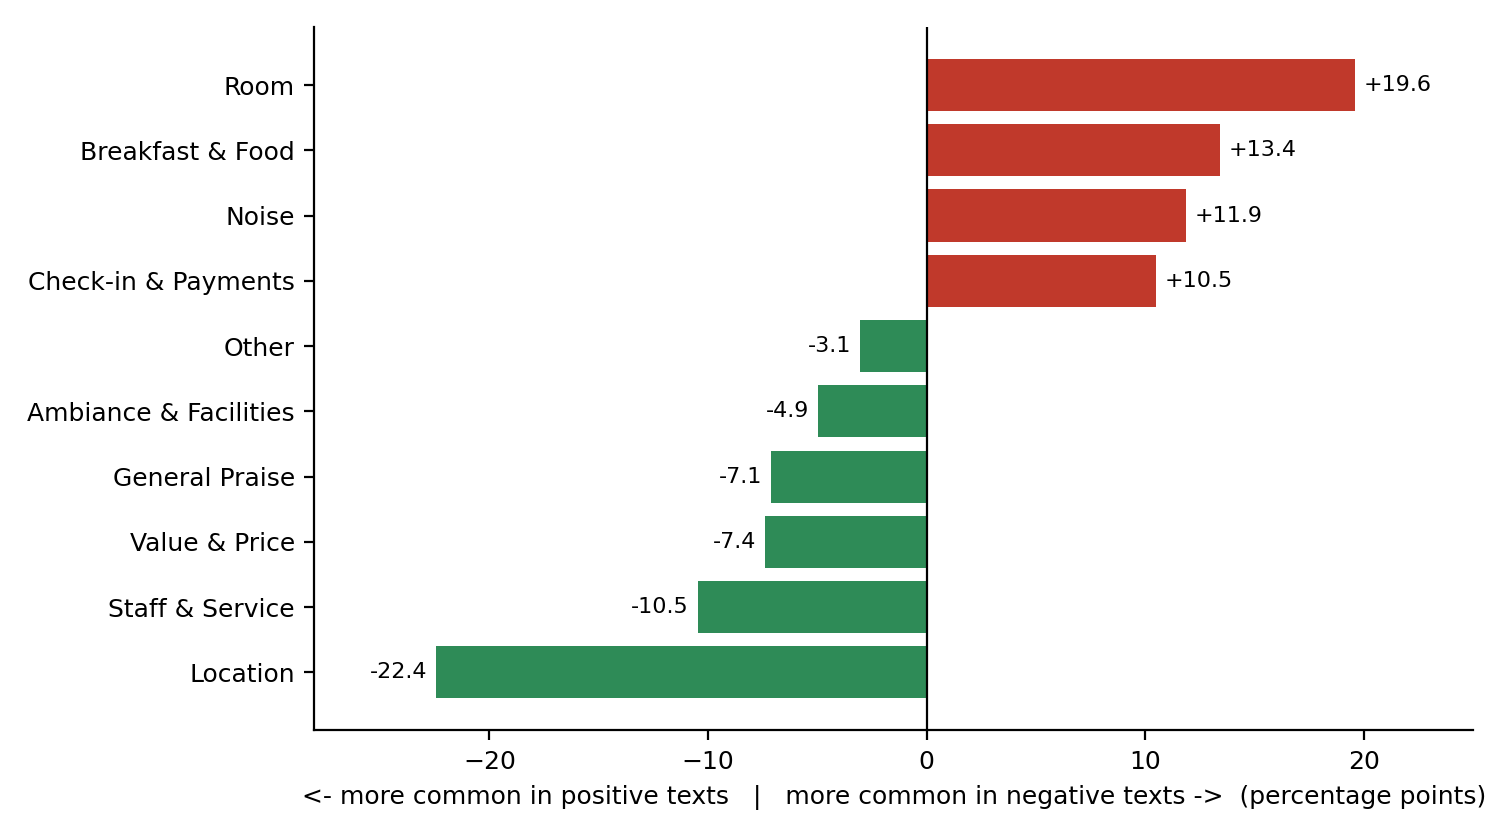
\includegraphics[width=0.92\linewidth]{fig_theme_difference.png}
\caption{Difference in theme share between negative and positive texts. Positive bars (red) mark complaint-heavy themes (hygiene-factor candidates), negative bars (green) praise-heavy themes (satisfaction-driver candidates).}
\label{fig:diff}
\end{figure}

\textbf{Hygiene factors.} Room quality is the largest source of complaints (30.2\% of negative texts) and is almost three times more prevalent in complaints than in praise ($R=2.84$). It combines bathroom condition with bed size, comfort and parking. Breakfast and food account for 18.8\% of complaints, 3.5 times their share of praise. Noise (11.9\%) and check-in, WiFi and payment issues (10.5\%) appear only among the complaint themes.

\textbf{Satisfaction drivers.} Location is the strongest driver of praise: 29.8\% of positive texts but only 7.4\% of negative texts ($R=0.25$). Staff and service is the second largest praise theme (25.1\%) but also accounts for 14.6\% of complaints, so it acts in both directions. Ambiance and facilities (11.5\% vs.\ 6.6\%) is a weaker driver of praise, and value for money and general praise appear only on the positive side.

\subsection{Failure Modes and Error Analysis}
Table~\ref{tab:fail} summarises the failure modes that were observed or can be anticipated, together with the evidence and the mitigation used or proposed.

\begin{table}[!t]
\caption{Failure modes, evidence and mitigation}
\label{tab:fail}
\centering
\footnotesize
\begin{tabular}{p{3.0cm}p{5.0cm}p{5.0cm}}
\toprule
Failure mode & Evidence & Mitigation \\
\midrule
Label noise from structure-derived labels & A negative-model topic made of ``nothing'', ``everything'', ``great'' (41,800 segments, 10.9\% of negative texts) & Topic identified and excluded; audit a manual sample and validate against reviewer score \\
Negation lost in preprocessing & The default NLTK stop-word list contains ``not'' and ``no'', so ``not clean'' reduces to ``clean'' & Keep negations in the stop-word list; build bigrams before stop-word removal \\
Redundant topics from an unvalidated $k$ & Two near-identical transit topics at $k=10$ & Select $k$ with a coherence sweep \\
Catch-all topics & ``Minor/mixed remarks'' has low word weights and generic words & Reported as ``Other''; excluded from interpretation \\
One topic per text & Dominant-topic assignment ignores multi-aspect reviews & Use the full topic distribution $\boldsymbol{\theta}_d$ in future work \\
One-sided themes from two models & Noise and check-in exist only in the negative model; price is absorbed into breakfast & Interpret as complaint themes, not as absent from praise; fit a joint model or aspect-based sentiment \\
Limited coverage & Six countries, 2015--2017, upper-segment hotels, mostly English text & State as a scope limitation; replicate on newer data \\
Single split on a sample & Classifier comparison uses one 30,000-segment test split & Use cross-validation and full-corpus evaluation \\
\bottomrule
\end{tabular}
\end{table}

\section{Discussion and Industrial Application}
\subsection{Interpretation}
The results are consistent with a two-factor view of satisfaction. Rooms, breakfast, noise and check-in behave like hygiene factors: they appear disproportionately when something goes wrong. Location behaves like a satisfaction driver: guests mention it mostly when they are pleased, and rarely as a complaint, which is natural because it is a fixed property of the hotel. Staff and service is the exception that matters most for management: it is simultaneously the second most common praise theme and a major source of complaints, which suggests that service quality can make or break a stay. These are associations between text themes and sentiment, not causal effects.

\subsection{Business Impact}
For a hotel operator, the analysis translates into a prioritised action list. Because room quality and breakfast together account for almost half of all complaint texts (49.0\%), maintenance of bathrooms, beds and breakfast quality and pricing are the most effective levers for reducing negative reviews. Noise and check-in issues are inexpensive to address: sound insulation or room-allocation rules, faster check-in and clearer payment and WiFi information. Location cannot be changed, but because it is the strongest source of praise it should be highlighted in marketing. Staff training addresses a theme that appears on both sides. At portfolio level, the same pipeline can rank properties by their complaint-theme mix to target renovation budgets.

\subsection{Deployment Architecture and Scalability}
The pipeline can be deployed as a batch job that ingests new reviews daily or weekly, cleans and classifies them with the stored vectoriser and model, assigns topics with the stored LDA models and updates a dashboard. Retraining of the topic models is needed only periodically. At the scale of this study the entire workflow runs on a laptop; at the scale of an international chain or a review platform (hundreds of millions of texts) the same design maps directly to a distributed stack. Apache Spark MLlib \cite{meng2016} provides tokenisation, stop-word removal, count vectorisation, IDF weighting, Logistic Regression, Naive Bayes, linear SVM and an LDA implementation, so each stage of Fig.~\ref{fig:pipeline} has a distributed counterpart. The main scalability challenges are (i) LDA training cost, which grows with tokens and topics, (ii) the memory footprint of vocabularies with millions of n-grams, (iii) monitoring concept drift, since vocabulary and topics change over time, and (iv) multilingual input, which requires language detection and language-specific preprocessing.

\subsection{Implementation Feasibility and Responsible Use}
The method relies on open-source libraries, runs on commodity hardware and needs no labelled training data, which makes it feasible for small and medium-sized hotels. Two practical points deserve attention. Topic labels are produced by a human reading the top words, so a short review step is required after each retraining. Data from review platforms are subject to platform terms of use, and personal attributes such as reviewer nationality should not be used to profile individuals; results should be reported in aggregated form in line with the EU General Data Protection Regulation.

\subsection{Limitations and Threats to Validity}
\emph{Construct validity:} labels are derived from the review form, not from independent annotation. The high classification accuracy shows that the two fields have distinct vocabularies, but it overstates the accuracy that would be obtained on free text that mixes positive and negative statements. \emph{Internal validity:} negation words were removed by the stop-word list, which can obscure the meaning of phrases such as ``not clean''; the classifier comparison uses a single stratified split of a 150,000-segment sample and library-default regularisation; and topic labelling is subjective. \emph{External validity:} the corpus covers six countries, a two-year period and one platform, and the vocabulary is dominated by English. \emph{Analytical validity:} the combined analysis relies on a manual mapping of topics to themes and on dominant-topic assignment; one-sided themes partly reflect the separation of the two topic models.

\section{Conclusion and Future Work}
This paper presented a reproducible pipeline that combines TF-IDF sentiment classification and sentiment-specific LDA topic modelling to identify the drivers of guest satisfaction in 515,738 European hotel reviews. Logistic Regression achieved the best macro-F1 (0.929) while remaining about twice as fast as the linear SVM, and Naive Bayes was the fastest model at a cost of about one percentage point in F1. Coherence-based selection yielded 13 topics for positive and 9 topics for negative texts. Mapping the topics to shared themes showed that room quality, breakfast and food, noise and check-in problems are over-represented in complaints, location is the dominant source of praise, and staff and service is important in both directions.

Future work follows directly from the limitations. First, labels should be validated against the overall reviewer score and a manually annotated sample, and negation should be preserved in preprocessing. Second, the comparison should be extended with cross-validation, tuned regularisation and transformer models such as BERT \cite{devlin2019}. Third, a joint or aspect-based model that estimates sentiment per aspect would remove the one-sided-theme problem, and using the full topic distribution of each text would replace the dominant-topic simplification. Fourth, the temporal dimension (trends and seasonality) and country-level differences can be analysed. Finally, the pipeline can be re-implemented on Apache Spark and exposed through an interactive dashboard for hotel managers.

\section*{Acknowledgment}
The author thanks the supervisors and colleagues for their feedback. The dataset is a public Booking.com extract hosted on Kaggle.

\appendices
\section{Reproducibility}
The repository accompanying this paper contains five notebooks that map one-to-one to the stages of Fig.~\ref{fig:pipeline}: (01) cleaning and preprocessing, (02) exploratory analysis, (03) sentiment classification, (04) topic modelling and (05) combined analysis. The figures of Section~VI can be regenerated from the stored results. The raw dataset is not redistributed; the README explains how to download it. Random seeds are fixed to 42 for the data split, the classifiers and the LDA models.

\begin{thebibliography}{99}
\bibitem{xiang2010} Z. Xiang and U. Gretzel, ``Role of social media in online travel information search,'' \emph{Tourism Management}, vol. 31, no. 2, pp. 179--188, 2010.
\bibitem{ye2009} Q. Ye, R. Law, and B. Gu, ``The impact of online user reviews on hotel room sales,'' \emph{Int. J. Hospitality Management}, vol. 28, no. 1, pp. 180--182, 2009.
\bibitem{guo2017} Y. Guo, S. J. Barnes, and Q. Jia, ``Mining meaning from online ratings and reviews: Tourist satisfaction analysis using latent Dirichlet allocation,'' \emph{Tourism Management}, vol. 59, pp. 467--483, 2017.
\bibitem{pang2002} B. Pang, L. Lee, and S. Vaithyanathan, ``Thumbs up? Sentiment classification using machine learning techniques,'' in \emph{Proc. Conf. Empirical Methods in Natural Language Processing (EMNLP)}, 2002, pp. 79--86.
\bibitem{wang2012} S. Wang and C. D. Manning, ``Baselines and bigrams: Simple, good sentiment and topic classification,'' in \emph{Proc. 50th Annu. Meeting Assoc. Computational Linguistics (Short Papers)}, 2012, pp. 90--94.
\bibitem{joachims1998} T. Joachims, ``Text categorization with support vector machines: Learning with many relevant features,'' in \emph{Proc. Eur. Conf. Machine Learning (ECML)}, 1998, pp. 137--142.
\bibitem{mccallum1998} A. McCallum and K. Nigam, ``A comparison of event models for naive Bayes text classification,'' in \emph{AAAI-98 Workshop on Learning for Text Categorization}, 1998, pp. 41--48.
\bibitem{salton1988} G. Salton and C. Buckley, ``Term-weighting approaches in automatic text retrieval,'' \emph{Inf. Process. Manage.}, vol. 24, no. 5, pp. 513--523, 1988.
\bibitem{liu2012} B. Liu, \emph{Sentiment Analysis and Opinion Mining}. San Rafael, CA, USA: Morgan \& Claypool, 2012.
\bibitem{devlin2019} J. Devlin, M.-W. Chang, K. Lee, and K. Toutanova, ``BERT: Pre-training of deep bidirectional transformers for language understanding,'' in \emph{Proc. NAACL-HLT}, 2019, pp. 4171--4186.
\bibitem{blei2003} D. M. Blei, A. Y. Ng, and M. I. Jordan, ``Latent Dirichlet allocation,'' \emph{J. Mach. Learn. Res.}, vol. 3, pp. 993--1022, 2003.
\bibitem{blei2012} D. M. Blei, ``Probabilistic topic models,'' \emph{Commun. ACM}, vol. 55, no. 4, pp. 77--84, 2012.
\bibitem{hoffman2010} M. Hoffman, F. R. Bach, and D. M. Blei, ``Online learning for latent Dirichlet allocation,'' in \emph{Adv. Neural Inf. Process. Syst. (NIPS)}, 2010, pp. 856--864.
\bibitem{mimno2011} D. Mimno, H. M. Wallach, E. Talley, M. Leenders, and A. McCallum, ``Optimizing semantic coherence in topic models,'' in \emph{Proc. EMNLP}, 2011, pp. 262--272.
\bibitem{roder2015} M. R\"oder, A. Both, and A. Hinneburg, ``Exploring the space of topic coherence measures,'' in \emph{Proc. 8th ACM Int. Conf. Web Search and Data Mining (WSDM)}, 2015, pp. 399--408.
\bibitem{rehurek2010} R. \v{R}eh\r{u}\v{r}ek and P. Sojka, ``Software framework for topic modelling with large corpora,'' in \emph{Proc. LREC Workshop on New Challenges for NLP Frameworks}, 2010, pp. 45--50.
\bibitem{pedregosa2011} F. Pedregosa \emph{et al.}, ``Scikit-learn: Machine learning in Python,'' \emph{J. Mach. Learn. Res.}, vol. 12, pp. 2825--2830, 2011.
\bibitem{fan2008} R.-E. Fan, K.-W. Chang, C.-J. Hsieh, X.-R. Wang, and C.-J. Lin, ``LIBLINEAR: A library for large linear classification,'' \emph{J. Mach. Learn. Res.}, vol. 9, pp. 1871--1874, 2008.
\bibitem{herzberg1959} F. Herzberg, B. Mausner, and B. B. Snyderman, \emph{The Motivation to Work}, 2nd ed. New York, NY, USA: Wiley, 1959.
\bibitem{bird2009} S. Bird, E. Klein, and E. Loper, \emph{Natural Language Processing with Python}. Sebastopol, CA, USA: O'Reilly Media, 2009.
\bibitem{meng2016} X. Meng \emph{et al.}, ``MLlib: Machine learning in Apache Spark,'' \emph{J. Mach. Learn. Res.}, vol. 17, no. 34, pp. 1--7, 2016.
\bibitem{liu2018dataset} J. Liu, ``515K hotel reviews data in Europe,'' Kaggle dataset. [Online]. Available: https://www.kaggle.com/datasets/jiashenliu/515k-hotel-reviews-data-in-europe
\end{thebibliography}

\end{document}
